\documentclass[12pt,a4paper]{report}
\usepackage{amsmath,amsthm,amssymb,mathrsfs,graphicx,comment,blindtext,subfiles,tikz}
\usepackage[noend]{algorithmic} %algorithmic environment
\usetikzlibrary{shapes.geometric,calc}
\allowdisplaybreaks


\newtheorem{theorem}{Theorem}[section]
\newtheorem{definition}[theorem]{Definition}
\newtheorem{example}[theorem]{Example}
\newtheorem{corollary}[theorem]{Corollary}
\newtheorem{lemma}[theorem]{Lemma}
\newtheorem{proposition}[theorem]{Proposition}
\newtheorem{remark}[theorem]{Remark}
\newtheorem{algorithm}[theorem]{Algorithm}

\renewcommand{\baselinestretch}{1.5}
\renewcommand{\algorithmicrequire}{\textbf{Input:}}
\renewcommand{\algorithmicensure}{\textbf{Output:}}

%% Replace init/inif with \initial or "in"
\DeclareMathOperator{\initial}{in}

\begin{document}

%TODO----------------------------------------------------------------------------------------------------------------------

%Roadmap until submission date: (25th)

%Chapter 1: Missing
%Chapter 2.1: missing examples and pictures - DONE
%Chapter 2.2: (missing examples) - DONE
%Chapter 3.1: missing examples and pictures - DONE (no pics?)
%Chapter 3.2: remove - DONE
%Merge Chapter 3+4 - DONE
%%Separate Tracking Progress chapter - DONE
%%DONE---------------------------------------------------------------
%(Chapter 4 feedback next Tuesday) - ALMOST DONE!!
%Chapter 5: improve structure (put definitions into definition environments, etc)
%Some remarks on Chapter 5:
%- missing: desired properties of a progress measure
%Failure type 1: it increases
%Failure type 2: it gets stuck
%Failure type 3: it becomes becomes the bottleneck
%From Yue Ren to Everyone:  01:27 PM
%Suggestion for structure of section 5:
%Section 5.1: facet oriented methods
%Section 5.2: line oriented methods
%5.1.1: Barycenter
%5.1.2: L1 Ball
%remark in 5.1.2: great circle distance

%%\appendix
%%\chapter{blablabla}
%missing in the merged chapter 3+4: survey of other Groebner walk methods


\chapter{diagram nonsense}
%%Chapter 2---------------------------------------------------------------------------------------------------------------

%%Example of a Not pure Not complete fan
\begin{figure}
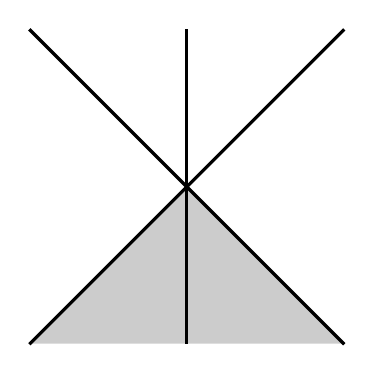
\begin{tikzpicture}
\draw[fill=black!20!white, draw=white] (0,0)--(-2,-2)--(0,-2)--(2,-2)--(0,0)--cycle;
\draw[very thick] (0,0) -- (0,2); %%Top
\draw[very thick] (0,0) -- (0,-2); %%Bottom
\draw[very thick] (0,0) -- (2,2); %%TopRight
\draw[very thick] (0,0) -- (-2,-2); %%BottomLeft
\draw[very thick] (0,0) -- (2,-2); %%BottomRight
\draw[very thick] (0,0) -- (-2,2); %%TopLeft


\end{tikzpicture}
\end{figure}

%Description
This collection of cones consists of: 1 zero-dimensional cone, 6 rays and 2 two-dimensional cones. This is a fan, however it is not complete (since the support of the fan is not $\mathbb{R^{2}}$), and it is not pure (since not all of its maximal cones have the same dimension).




%%Example of a pure Not complete fan
\begin{figure}
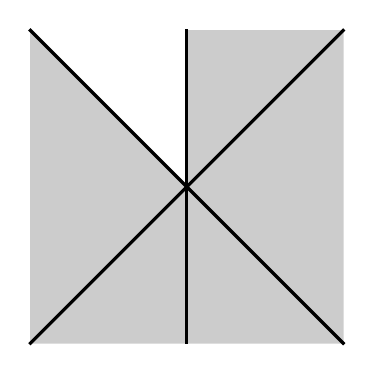
\begin{tikzpicture}

\draw[fill=black!20!white, draw=white] (0,0)--(-2,2)--(-2,-2)--(0,-2)--(2,-2)--(2,2)--(0,2)--cycle;
\draw[very thick] (0,0) -- (0,2);
\draw[very thick] (0,0) -- (0,-2);
\draw[very thick] (0,0) -- (2,2);
\draw[very thick] (0,0) -- (-2,-2);
\draw[very thick] (0,0) -- (2,-2);
\draw[very thick] (0,0) -- (-2,2);

\end{tikzpicture}
\end{figure}

%Description
This collection of cones consists of: 1 zero-dimensional cone, 6 rays and 5 two-dimensional cones. This is a fan and it is not complete (since the support of the fan is not $\mathbb{R^{2}}$), but it is pure (all maximal cones have same dimension).

%%Example of a pure complete fan
\begin{figure}
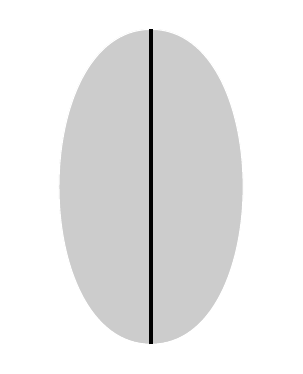
\begin{tikzpicture}
\coordinate (A) at (0,-2);
\coordinate (B) at (0, 2);

\draw[fill=black!20!white, draw=white] (A) to [bend left=90] (B);
\draw[fill=black!20!white, draw=white] (A) to [bend right=90] (B);
\draw[very thick] (A)--(B);
\end{tikzpicture}
\end{figure}

%Description
This collection of cones consists of: 1 line and two regions. This is a fan and it is both complete and pure.

%%Example of a NOT fan
\begin{figure}
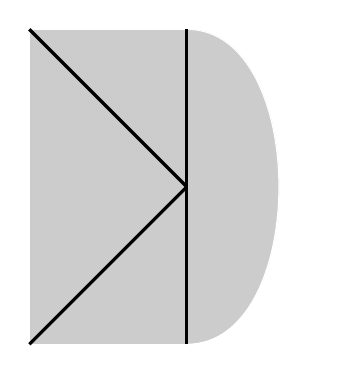
\begin{tikzpicture}
\coordinate (A) at (0,-2);
\coordinate (B) at (0, 2);

\draw[fill=black!20!white, draw=white] (A) to [bend right=90] (B);
\draw[fill=black!20!white, draw=white] (0,0)--(0,2)--(-2,2)--(-2,-2)--(0,-2)--cycle;
\draw[very thick] (A)--(B);
\draw[very thick] (0,0) -- (-2,2); %%TopLeft
\draw[very thick] (0,0) -- (-2,-2); %%BottomLeft
\end{tikzpicture}
\end{figure}

%Description
This collection of cones consists of: 1 zero-dimensional, 4 rays, one line and 4 regions, one of which is a half-space. The existence of this half-space means that this is not a polyhedral fan, due to the fact that intersections of other regions with this half-space is not a face of the same half-space.

Relative interior is a refinement of the concept of interior, and is useful for dealing with lower-dimensional sets in higher-dimensional spaces. An example of this is the set of points $(x, y, 0)$ restricted by $x^2 + y^2 \leq 1$ in $\mathbb{R}^{3}$. If we take the interior of this set, we find that the interior is empty. It is empty due to how interior is defined i.e. a point $p$ is in the interior if we can construct an open ball around $p$, and the open ball is itself contained within the set. In the example outlined earlier, any open ball drawn around $p = (x, y, 0)$ will involve points that do not lie on the $xy$-plane. Hence, no points cannot be in the interior, and so it is empty.

While this is perfectly correct, its not really useful and fails to capture any information. By using relative interior, we instead look at the affine subspace, which is $\mathbb{R}^{2}$ (not $\mathbb{R}^{3}$), and so we construct open balls only in the $xy$-plane and ignore the $z$ dimension. This means that the relative interior is, instead of being empty, is the interior of the unit disc, as we would expect.  

%%Cite for Chapter 2.1 and Chapter 2.2 DONE!!

%%Redo < and \prec for order/preorder 


Lets try something:
\begin{figure}
\begin{center}
    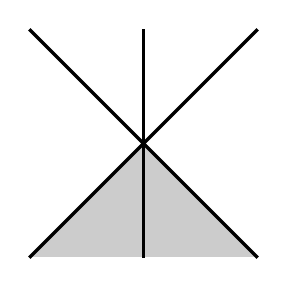
\begin{tikzpicture}[scale=0.725]
\draw[fill=black!20!white, draw=white] (0,0)--(-2,-2)--(0,-2)--(2,-2)--(0,0)--cycle;
\draw[very thick] (0,0) -- (0,2); %%Top
\draw[very thick] (0,0) -- (0,-2); %%Bottom
\draw[very thick] (0,0) -- (2,2); %%TopRight
\draw[very thick] (0,0) -- (-2,-2); %%BottomLeft
\draw[very thick] (0,0) -- (2,-2); %%BottomRight
\draw[very thick] (0,0) -- (-2,2); %%TopLeft
\end{tikzpicture} %%First image
\qquad
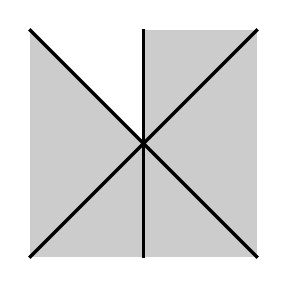
\begin{tikzpicture}[scale=0.725]
\draw[fill=black!20!white, draw=white] (0,0)--(-2,2)--(-2,-2)--(0,-2)--(2,-2)--(2,2)--(0,2)--cycle;
\draw[very thick] (0,0) -- (0,2);
\draw[very thick] (0,0) -- (0,-2);
\draw[very thick] (0,0) -- (2,2);
\draw[very thick] (0,0) -- (-2,-2);
\draw[very thick] (0,0) -- (2,-2);
\draw[very thick] (0,0) -- (-2,2);
\end{tikzpicture} %%Second image
\qquad
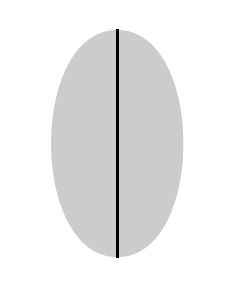
\begin{tikzpicture}[scale=0.725]
\coordinate (A) at (0,-2);
\coordinate (B) at (0, 2);
\draw[fill=black!20!white, draw=white] (A) to [bend left=90] (B);
\draw[fill=black!20!white, draw=white] (A) to [bend right=90] (B);
\draw[very thick] (A)--(B);
\end{tikzpicture} %%Third image
\qquad
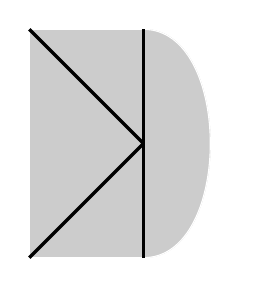
\begin{tikzpicture}[scale=0.725]
\coordinate (A) at (0,-2);
\coordinate (B) at (0, 2);
\draw[fill=black!20!white, draw=white] (A) to [bend right=90] (B);
\draw[fill=black!20!white, draw=white] (0,0)--(0,2)--(-2,2)--(-2,-2)--(0,-2)--cycle;
\draw[very thick] (A)--(B);
\draw[very thick] (0,0) -- (-2,2); %%TopLeft
\draw[very thick] (0,0) -- (-2,-2); %%BottomLeft
\end{tikzpicture}
\end{center}
\caption{A collection of 4 different cones referenced in PLACEHOLDER}
\end{figure}


%%Chapter 3---------------------------------------------------------------------------------------------------------------

%%Chapter 5-----------------------------------------------------------
Instead of writing the "measuring distance" conditions in these terms, we can rewrite them in terms of failure states.
\begin{itemize}
    \item Failure type 1: The distance measuring function increases when performing step(s) of the Groebner Walk.
    \item Failure type 2: The distance measuring function gets stuck when performing the Groebner Walk.
    \item Failure type 3: The distance measuring function becomes a computational bottleneck.
\end{itemize}
This is similar to our two conditions above




\begin{figure}
\begin{tikzpicture}[scale=1.5]
% Draw axes
\draw [<->,thick] (0,3) node (yaxis) [above] {$y$}
    |- (3,0) node (xaxis) [right] {$x$};
    
\draw[thick,dotted] (2,0)--(0,2);
  \node[blue,anchor=west] at (0.5,2) {$|x| + |y| = 1$};
\end{tikzpicture}
\end{figure}



\end{document}
